\listoftodos



\chapter{Grundlagen}
\label{chap:Grundlagen}

	\section{TODO GRUNDALGENDETAIL}
	\label{sec:TODOGrundlagenDetail}
		\todo{notwendige klassische Grundlagen definieren} 
		
	\section{Einordnung und bestehende Systeme}
	\label{sec:BestehendesSystem}
	Die Bilddaten und Aufgabenstellungen der neuronalen Netzwerke sind in die Problemstellungen des Autocrane-Projekts von PSIORI einzuordnen. Es sind also echte Datensätze und echte Problemstellungen, wobei die gezeigten Aufgabenstellungen und Modelle nicht zwingend in dem Autocrane-Projekt zum Einsatz kommen. Das Autocrane-Projekt ist ein laufendes Projekt, welches das Ziel hat, einen feststehenden Rundlaufkran vollautomatischen zu steuern. In Abbildung \ref{img:CircularCrane} ist ein Rundlaufkran abgebildet. Dieser Kran wird in einer holzverarbeitenden Anlage zum Befüllen eines Fülltrichters eingesetzt. Dabei sind insbesondere drei Anwendungsfälle interessant. Die Baumstämme werden mittels LKW angeliefert und müssen nach vorgegebenen Regeln (z. B. Ausrichtung, freier Lagerplatz) als Holzstapel gelagert werden. Der Fülltrichter muss mit Holz aus den Holzstapeln oder vom LKW aus befüllt werden. Es ergeben sich also Aufgabenstellungen wie Greifer-Erkennung, Baumstamm-Erkennung, LKW-Erkennung, Strategien für das entladen und aufbewahren der Baumstämme und vieles mehr.	\todo{Quelle Doku PSIORI}
	\begin{figure}[h]
		\centering
		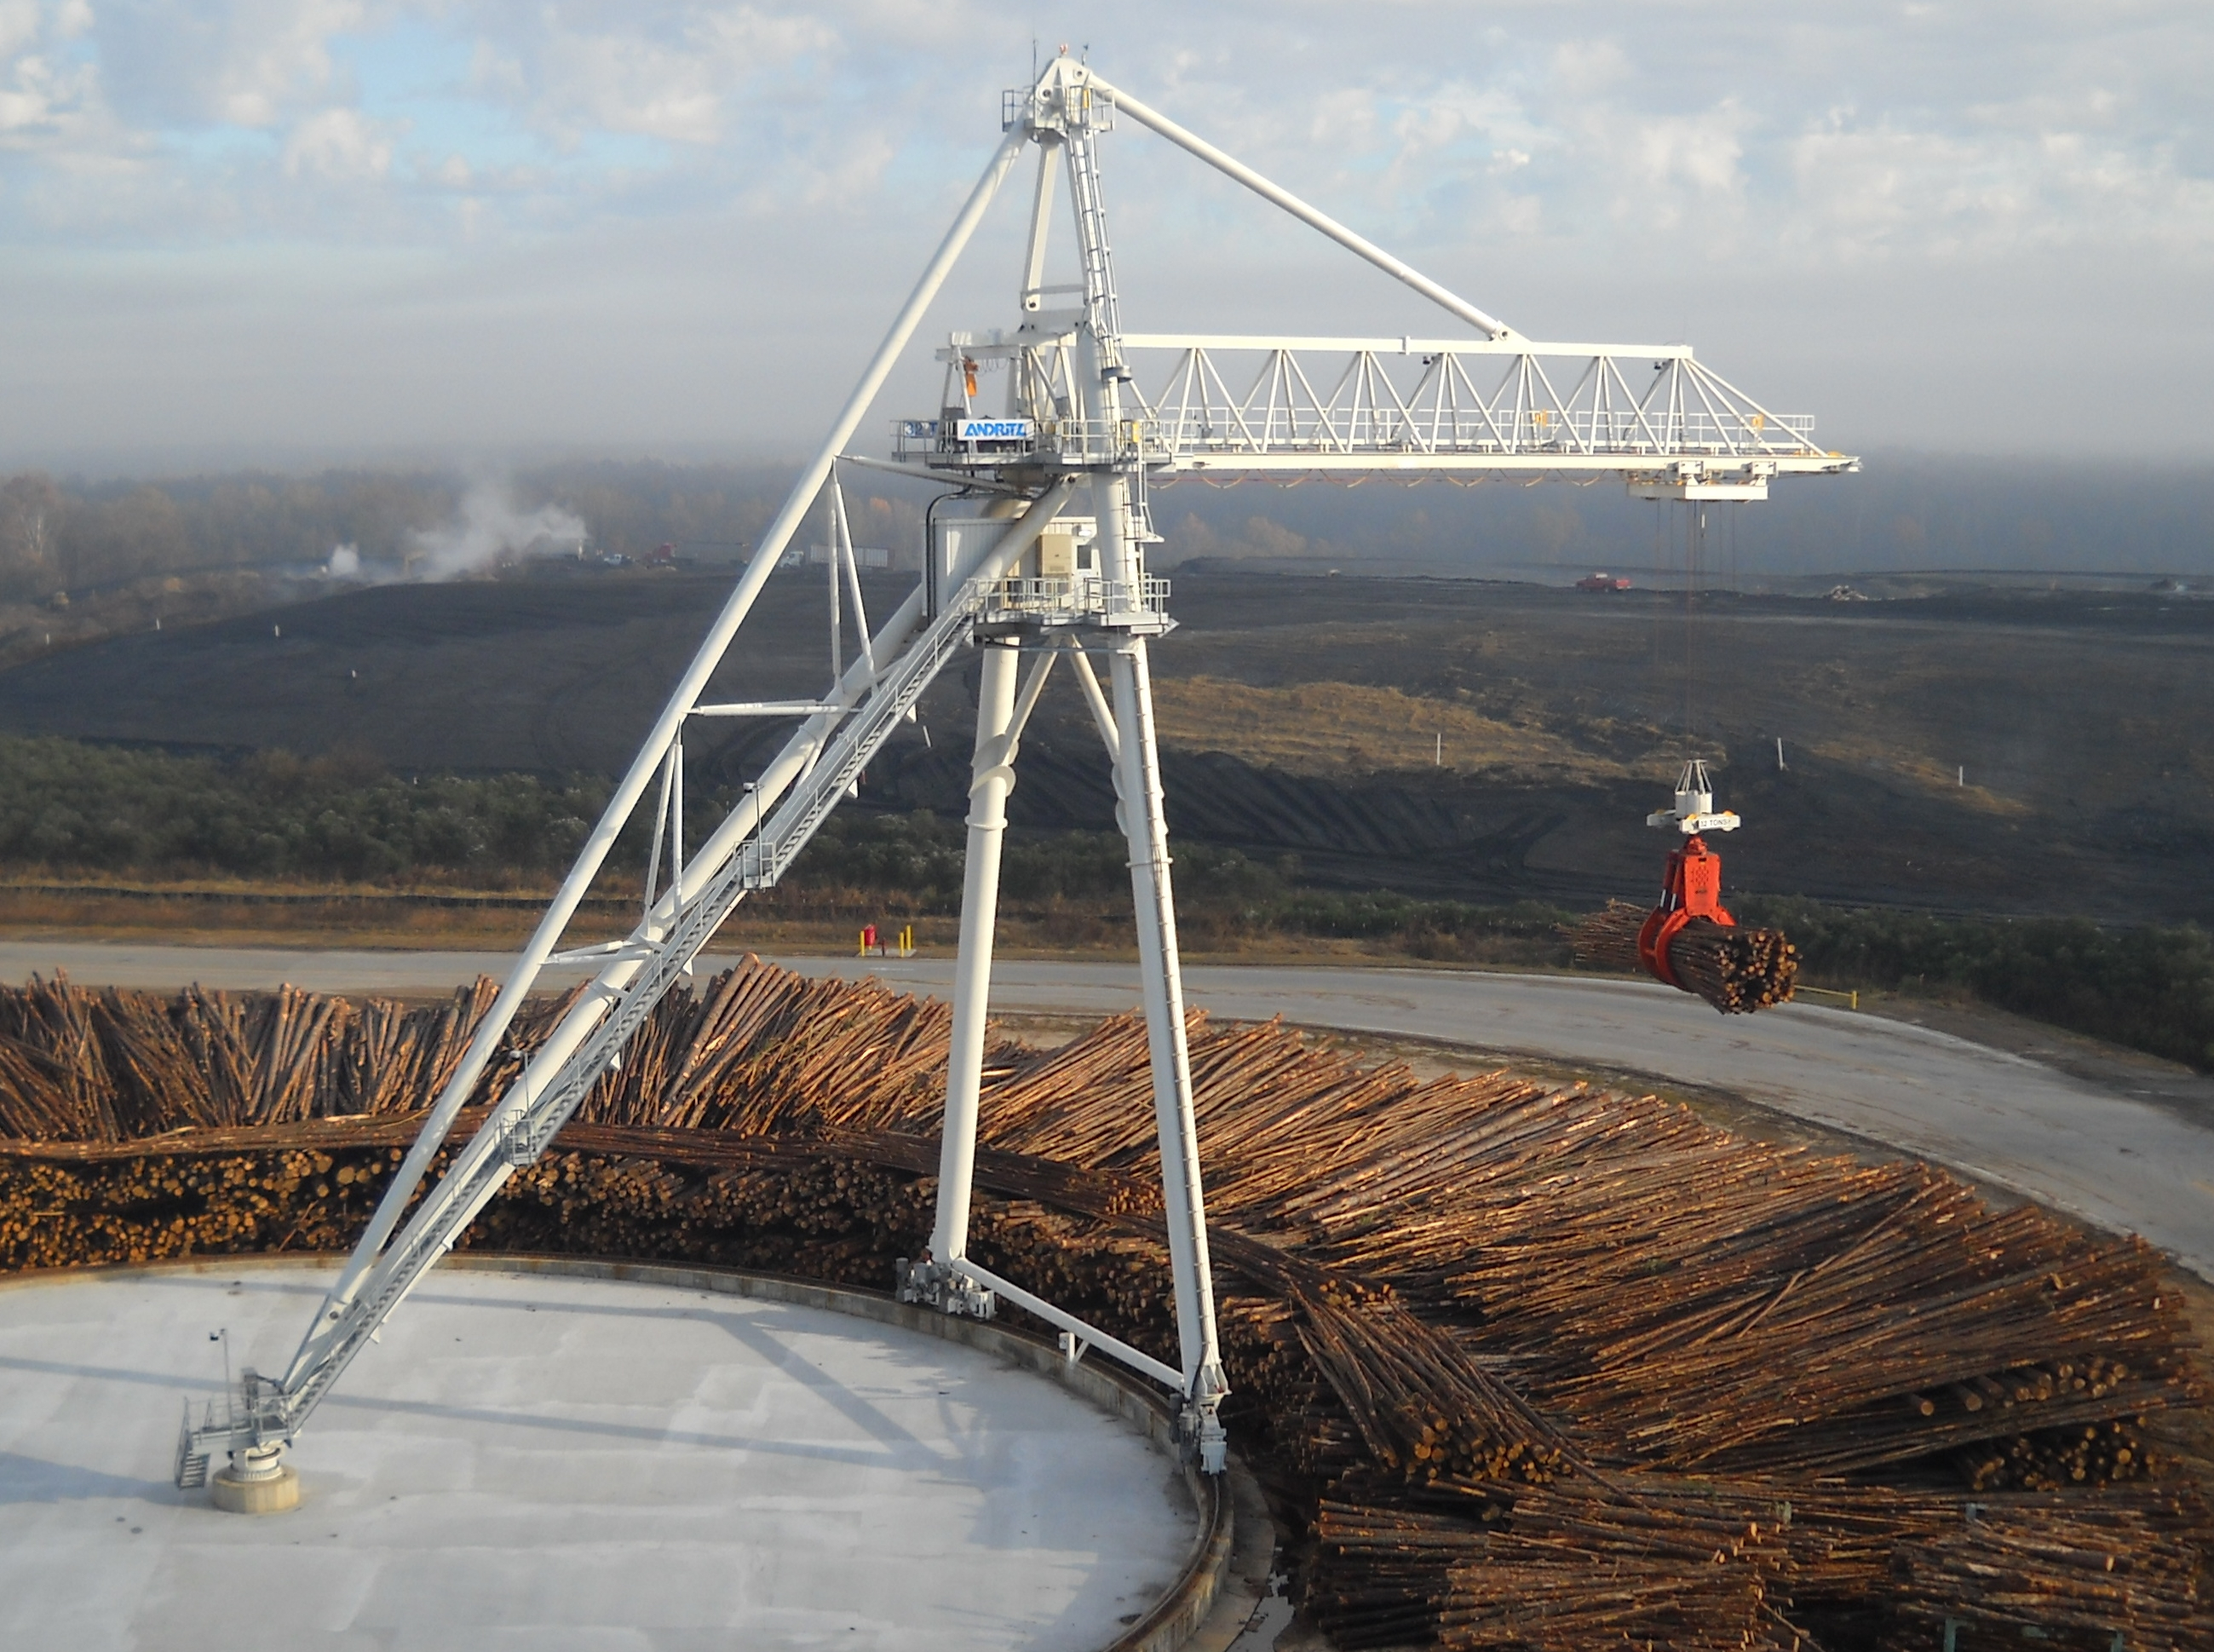
\includegraphics[width=0.5\textwidth, center]{bilder/Grundlagen/Kran_vollstaendig_N1_030.jpg}
		\caption[Rund-Kran]{Rundlaufkran (Foto: ANDRITZ)}
		\label{img:CircularCrane}
	\end{figure}		
	\paragraph{Greifer-Erkennung} Model erläutern 

	\section{Datenverständnis}
	\label{sec:DataUnderstanding}
	Anlehnend dem in Kapitel \ref{sec:Vorgehen} beschriebenen Vorgehen \todo{Vorgehen auch so beschreiben /  ansonsten Kapitel Einleitung anpassen} werden in diesem Kapitel die zur Verfügung stehenden Daten und deren Qualität beschrieben. Dabei ist das Kapitel entsprechend der Beschriftung der Daten in zwei Teilbereiche unterteilt.
	
	Im Rahmen des Autocrane-Projektes \ref{sec:BestehendesSystem} \todo{Im Kapitel Bestehdens System erwähnen / diesen Teil in das andere Kapitel verschieben?} wurde eine Kamera an einem Rundlaufkran angebracht. Die Kamera ist so ausgerichtet, dass sich Aufhängung des Greifers am mittleren oberen Bildrand befindet. Bei einem Rundlaufkran kann die Auslenkung komplett um das Zentrum des Krans bewegt werden. Der Hintergrund der Bilder kann sich stark ändern. Mittels der Kamera werden kontinuirlich neue unbeschriftete Bilder aufgenommen und bei PSIORI abgelegt. Zu Beginn dieser Arbeit standen mehr 385.000 nicht beschriftete Bilder zur Verfügung. Die Bilder sind 1024 auf 648 Pixel groß und in Farbe. Sie sind in der Form (1024, 648, 3). Die einzelnen Pixel können dabei Werte zwischen 0 und 255 annehmen. 
	Zum Erreichen der Zielstellung werden zwei Datensätze benötigt.
	
		\paragraph{Greifer Datensatz} Der Greifer Datensatz enthält Bilder, in welchen der Greifer mittels Rahmen markiert ist. Abbildung \ref{img:Logs}  zeigt ein beispielhaftes Bild mit markiertem Greifer. Abbildung \ref{img:Grapple} zeigt ein beispielhaftes Bild mit markiertem Greifer.
		\begin{figure}[h]
				\centering
				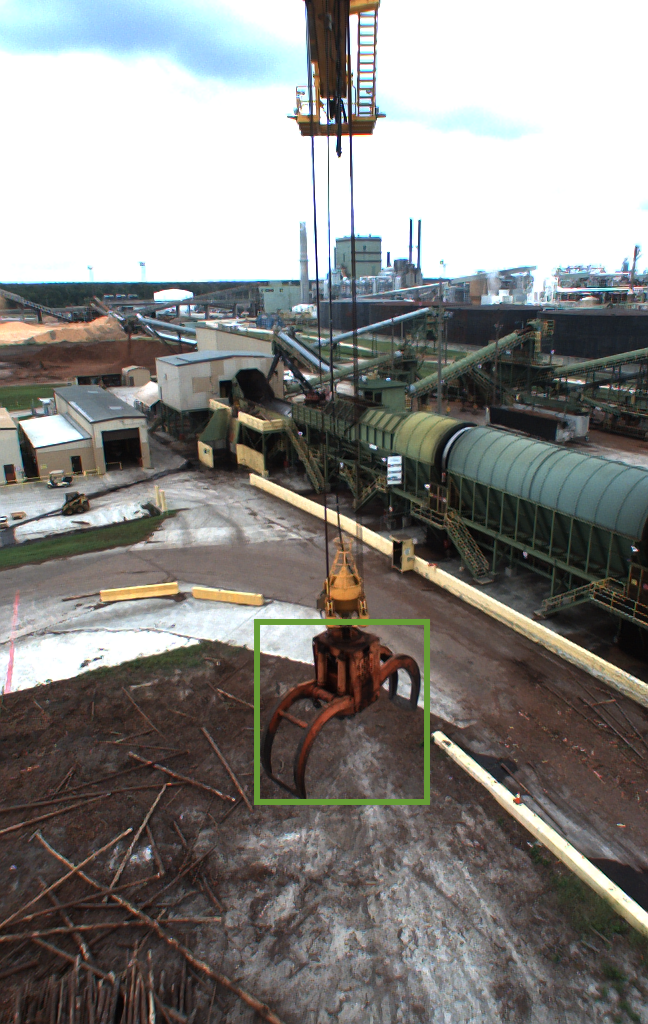
\includegraphics[width=0.5\textwidth, center]{bilder/Grundlagen/Grapple_8.png}
				\caption[Bsp. Bild: Greifer mit Rahmen]{Greifer mit Rahmen}
				\label{img:Grapple}
		\end{figure}
		Der Datensatz besteht aus zwei Sammlungen von qualitativ unterschiedlich gut beschrifteten Bildern. Die eine Sammlung besteht aus einem bestehenden Datensatz, welcher 4.684 durch Menschen annotierten Bildern enthält. Für den zweiten Teil der Sammlung wurden mittels der \todo{siehe Bestehendes System} bestehenden Objekterkennung XXXX Bilder annotiert. \todo{Vorgehen + Metriken detailierter beschreiben} Das genaue Schema der Datenstrukturen kann in Anhang \ref{appendix:AutocraneDaten} nachgelesen werden.

		\paragraph{Baumstamm Datensatz} Der Baumstamm Datensatz enthält Bilder, welche die Annotation, ob sich Baumstämme im Greifer befinden haben. Abbildung \ref{img:Logs} zeigt ein Bild, in welchem der Greifer Baumstämme greift. In Abbildung \ref{img:Grapple} befinden sich keine Baumstämme im Greifer.
		\begin{figure}[h]
			\centering
			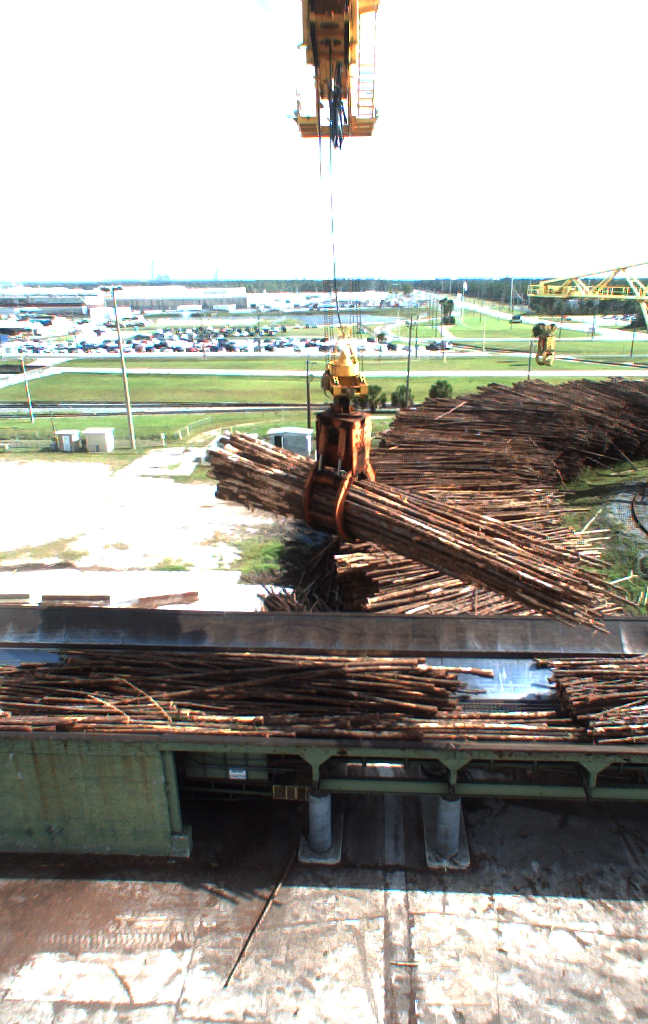
\includegraphics[width=0.5\textwidth, center]{bilder/Grundlagen/Logs_14.png}
			\caption[Bsp. Bild: Greifer mit Baumstämmen]{Greifer mit Baumstämmen}
			\label{img:Logs}
		\end{figure}
		Der Datensatz wurde mittels Crowd
			
	%		\begin{figure}[h]
	%		\centering
	%		\includegraphics[width=0.5\textwidth, center]{bilder/Grundlagen/.png}
	%		\caption[Bsp. Bild: Greifer mit Baumstämmen]{Greifer mit Baumstämmen}
	%		\label{img:Helligkeit}
	%		\end{figure}			
		

				
		 \todo{Brightness-Histogramm einfügen} 
			
				 Im Rahmen des Datenverständnisses wird versucht, sich einen ersten Überblick über die zur Verfügung stehenden Daten und deren Qualität zu verschaffen. Es erfolgt eine Analyse und Bewertung der Datenqualität. Probleme mit der Qualität der vorhandenen Daten in Bezug auf die in der vorherigen Phase festgelegten Aufgabenstellung sind zu benennen.
			
			todo? Datenqualität auf helle und dunkle bidler verweisen und somit zu Datenvorbereitung: skalierung 0-1 verweissen
		
	\section{Datenvorbereitung}
	\label{sec:DataPreparation}

Die Datenvorbereitung dient dazu, einen finalen Datensatz zu erstellen, der die Basis für die nächste Phase der Modellierung bildet.


			In dem Schritt Datenvorbereitung werden die Bilder für die Modellerstelung vorbereitet. In dieser Arbeit wurde für diesen Schritt eine Klasse Preprocessing in einem neuen Modul data\_preperation.py  erstellt. Wie in Listing 
			% \lstinputlisting[language=Python,caption={Preprocessing},label=lst:Preprocessing]{\srcloc/data\_preperation.py }
			
			 zu sehen werden die Pixel der Bilder zwischen 0 und 1 Skaliert. Dei Skalierung erfolgt damit jedes Bild eine ähnliche Gewichtung
			
			Neural networks process inputs using small weight values, and inputs with large integer values can disrupt or slow down the learning process. As such it is good practice to normalize the pixel values so that each pixel value has a value between 0 and 1.
			
			Die Bilddaten werden 		
			
			\todo{Pretrain erläutern}

 

	\begin{table}[ht]
	\centering
	\begin{tabularx}{\textwidth}{lllll}
		 & \textbf{Train} & \textbf{Test}  & \textbf{Validation} & \textbf{Summe} 								  \\
		\textbf{Greifer} 				 & 	X					&	X					& 4.684 				   & x 				\\
		\textbf{Baumstämme T/F}	 	  &  X					 &	X					 &	X							& 18000		\\
	\end{tabularx}
	\caption{Datenaufteilung - Train Test Validation}
	\label{table:DatenaufteilungTrainTestValidation}
 	\end{table}
 
	\section{Bibliotheken und Werkzeuge}
	\label{sec:BibliothekenundWerkzeuge}
		\todo{TF + Keras nur per Ref}
		\paragraph{Tensorflow}
		\paragraph{Keras}
		
		
		\subsection{Psipy}
		\label{subsec:Psipy}
			Psipy ist ein Python-Framework für Maschinelles Lernen welches von PSIORI selbst entwickelte Modelle zusammenfasst und eine einheitliche API zu Verfügung stellt. Diese API ist an die API des verbreiteten Frameworks scikit-learn angelehnt und die Modelle aus scikit-learn können in das von PSIORI entwickelte Framework eingebunden werden. Das Framework ermöglicht außerdem das Einbinden von Modellen basierend auf TensorFlow.\grqq [PSIORI]
			
			PSIORI hat im Rahmen des Projektes ein Python-Framework für Maschinelles Lernen entwickelt, das von PSIORI selbst entwickelte Modelle zusammenfasst und eine einheitliche API zu Verfügung stellt. Diese API ist an die API des verbreiteten Frameworks scikit-learn [1] angelehnt und das PSIORI Framework ist mit scikit-learn insofern kompatibel, dass Modelle aus scikit-learn eingebunden werden können. Das Framework ermöglicht außerdem das Einbinden von Modellen basierend auf TensorFlow. [2]
			
		\paragraph{autoencoder.py}
			ConvolutionalAutoencoder 
			StackedAutoencoder
		\paragraph{call\_picky}
		\paragraph{hyperparameter\_mixin.py} 
			%	CS	https://automl.github.io/ConfigSpace/master/index.html# @article{
		%		title   = {BOAH: A Tool Suite for Multi-Fidelity Bayesian Optimization & Analysis of Hyperparameters},
		%		author  = {M. Lindauer and K. Eggensperger and M. Feurer and A. Biedenkapp and J. Marben and P. Müller and F. Hutter},
		%		journal = {arXiv:1908.06756 {[cs.LG]}},
		%		date    = {2019},
		%	}
		
		Für den effektiven Umgang mit Hyperparametern wurde das Open-Source-Paket ConfigSpace [5] eingebunden. Mithilfe dieses Pakets spannen die n Hyperparameter des Modells einen n-dimensionalen Raum auf, aus dem Modell-Konfigurationen gezogen, auf das Model angewandt und bezüglich eines Gütemaßes evaluiert werden können. Die Hyperparameter können dabei kontinuierlich in einem Intervall, kategorisch oder auch konstant sein. Je nach Art des jeweiligen Hyperparameters ist der Raum in der zugehörigen Dimension entweder kontinuierlich oder diskret und hat feste Grenzen. ConfigSpace erlaubt zudem die Anwendung von bestimmten Bedingungen und Regeln bezüglich der Werte, die ein Hyperparameter - gegebenenfalls in Abhängigkeit von anderen Hyperparametern - annehmen kann. Der Hyperparameter-Raum eines Modells bildet die Grundlage für alle implementierten Optimierungsalgorithmen, die im Folgenden beschrieben werden.
		
		\paragraph{hyperparameter\_optimization.py} 
Von den klassischen Suchverfahren zur Hyperparameteroptimierung wurden Algorithmen für Gittersuche und zufällige Suche implementiert, sodass sie insbesondere auf den Fully Connected Autoencoder angewendet werden können. Die gierige Suche wurde bisher nicht implementiert. Für die Gittersuche wird der von den Hyperparametern aufgespannte Raum entlang aller Dimensionen, d.h. Hyperparametern, diskretisiert, so das ein Gitter von gleichmäßig verteilten Hyperparameter-Kombinationen (Modell-Konfigurationen) entsteht. Die Gittersuche eignet sich vor allem bei einer kleinen Anzahl von Hyperparametern, da der Rechenaufwand mit der Zahl der Hyperparameter exponentiell ansteigt. Oft soll jedoch nur ein Teil der Hyperparameter optimiert werden, wodurch die Gittersuche sich als ein Standardverfahren in der Hyperparametersuche etabliert hat. [6]
Bei der zufälligen Suche werden Konfigurationen aus dem Hyperparameter-Raum zufällig gezogen und evaluiert. Die zufällige Suche ist in der Regel effizienter als die Gittersuche [6], garantiert jedoch keine Abdeckung des gesamten Hyperparameter-Raums.
Gitter- als auch zufällige Suche wurden für PsiPy als naive Standardverfahren sowie als mögliche Referenz für die Evaluation von neuen Algorithmen implementiert. Die gierige Suche wurde bisher nicht implementiert, da potentielle Anwendungsbereiche bereits von den anderen Suchverfahren hinreichend gedeckt sind.

Das State-of-the-Art-Verfahren zur Hyperparameteroptimierung, “Bayesian Optimization + Hyperband” (BOHB) [7] wurde in das entwickelte Framework eingebunden und kann mit dem Fully Connected Autoencoder genutzt werden. BOHB verbindet die Methoden Hyperband und Bayessche Optimierung. Hyperband erlaubt es, schnell eine vergleichsweise gute Konfiguration zu finden - ein häufiges Ziel, wenn z.B. verschiedene Modelle verglichen werden sollen. Da hier der Aufwand für die Evaluation einer Konfiguration davon abhängt, wie vielversprechend eine Konfiguration zu sein scheint, kann mit BOHB eine wesentlich effizientere Suche durchgeführt werden. Die Methode liegt als Open-Source-Paket [8] vor und wurde daher nicht neu implementiert. Das Paket bietet zudem die Möglichkeit zur Parallelisierung des Optimierungsprozesses, welche für den Fully Connected Autoencoder jedoch bisher nicht implementiert ist.


[6] Bergstra, James, and Yoshua Bengio. "Random search for hyper-parameter 
optimization." Journal of Machine Learning Research 13.Feb (2012): 281-305.
URL: http://www.jmlr.org/papers/volume13/bergstra12a/bergstra12a.pdf
[7] Falkner, Stefan, Aaron Klein, and Frank Hutter. "BOHB: Robust and efficient 
hyperparameter optimization at scale." arXiv preprint arXiv:1807.01774 (2018).
URL: https://ml.informatik.uni-freiburg.de/papers/18-ICML-BOHB.pdf 
[8] https://github.com/automl/HpBandSter

		
	\todo{Bild nur bestehendes System (Stacked Autoencoder + MixedHyperparam* )}
			\begin{figure}[h]
			\centering
			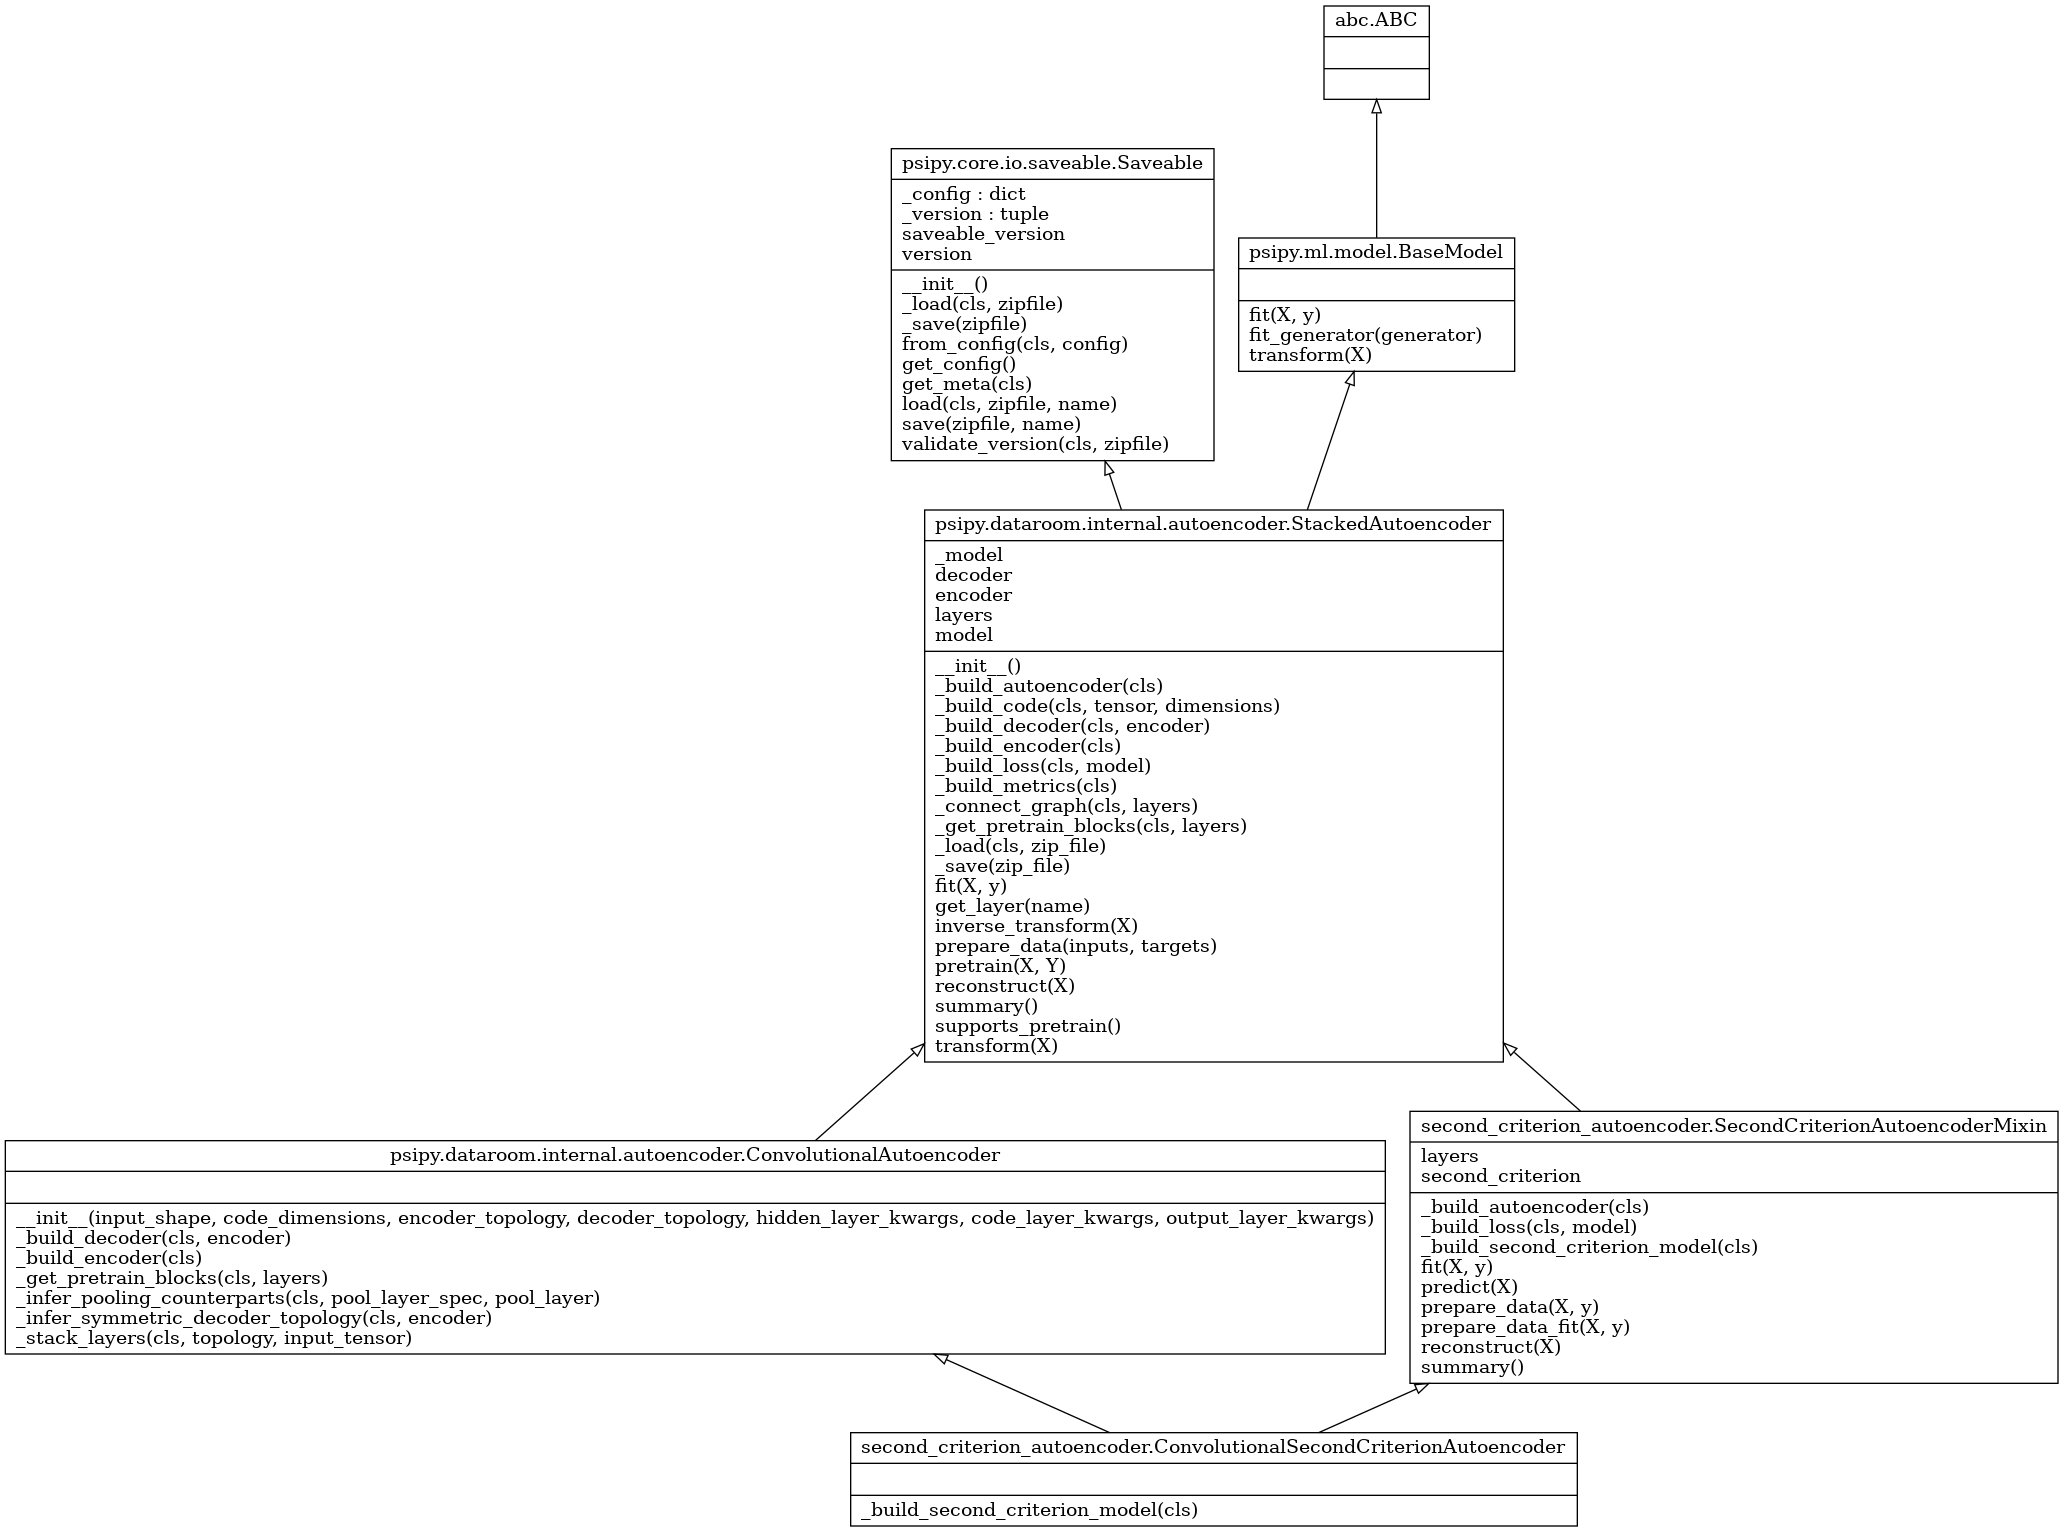
\includegraphics[width=\textwidth, center]{bilder/Grundlagen/Klassen_CSCA.png}
			\caption[Klassendiagramm ConvolutionalSecondCriterionAutoencoder]{Klassendiagramm ConvolutionalSecondCriterionAutoencoder}
			\label{img:ConvolutionalSecondCriterionAutoencoder}
		\end{figure}
		
		
		\subsection{Cnvrg.io}
		\label{subsec:Cnvrg.io}
		Cnvrg.io  \todo{Quelle cnvrg} ist eine "full-stack Data Science Platform" welche Werkzeuge  für die Erstellung, Verwaltung, Bereitstellung  und Automatisierung von maschinellem Lernen bereitstellt. \todo{mehr Text; was wurde genutzt (Datasets,...)}
			
	\section{Experimentumgebung}
	\label{sec:Experimentumgebung}
		(Hardware + eingesetzte Software)